\documentclass[9pt]{beamer}

\mode<presentation> {\usetheme{Kaiping}}
\setbeamercovered{transparent}

\usepackage[english]{babel}

\usepackage{fontspec}
\setmainfont{Linux Biolinum}
\setmonofont{DejaVu Sans Mono}
%\setsansfont{Linux Biolinum}
\newfontfamily{\fallbackfont}{DejaVu Sans}[Scale=MatchLowercase]
\DeclareTextFontCommand{\textfallback}{\fallbackfont}
\usepackage{newunicodechar}
\newunicodechar{⚀}{\fallbackfont{⚀}}
\newunicodechar{⚁}{\fallbackfont{⚁}}
\newunicodechar{⚂}{\fallbackfont{⚂}}
\newunicodechar{⚃}{\fallbackfont{⚃}}
\newunicodechar{⚄}{\fallbackfont{⚄}}
\newunicodechar{⚅}{\fallbackfont{⚅}}
\newunicodechar{ɛ}{\fallbackfont{ɛ}}
\newunicodechar{ʋ}{\fallbackfont{ʋ}}
\newunicodechar{ː}{\fallbackfont{ː}}

\usepackage{contour}
\usepackage{graphicx}
\usepackage{xcolor}
\usepackage{colortbl}
\usepackage{tikz}
\usepackage{tikz-cd}
\usetikzlibrary{trees,positioning,arrows}
\usetikzlibrary{automata}

\usepackage{listings}

\usepackage[style=authoryear,
            backend=biber,
            bibstyle=biblatex-sp-unified,
            citestyle=sp-authoryear-comp,
            maxcitenames=3,
            maxbibnames=99]{biblatex}
\bibliography{papers}
\newcommand{\paragraph}[1]{\par{\bfseries #1}}

\usefonttheme[onlymath]{serif}
\usetheme{Warsaw}
% default
% Boadilla
% Madrid
% Pittsburgh
% Rochester \usetheme[height=7mm]{Rochester}
% Copenhagen
% Warsaw
% Singapore
% Malmoe

\setlength{\parskip}{1ex plus 0.2ex minus 0.5ex}
\newcommand{\trees}{%
  \begin{tikzpicture}[sibling distance=3mm,level distance=3mm,
      every node/.style={align=center},
      node/.style={circle, fill, minimum size=0.3em,scale=0.3}]
    \node[node] (1) {}
    child { node[node] {}
      child { node[node] {}
        child { node[node] {} }}};
    \node[below=of 1]   {$\frac{8}{27}$\\\tiny$29.6\%$};
    \node[node,right=6mm of 1] (2) {}
    child { node[node] {}
      child { node[node] {}
        child { node[node] {} }
        child { node[node] {} }}};
    \node[below=of 2]   {$\frac{4}{27}$\\\tiny$14.8\%$};
    \node[node,right=6mm of 2] (3) {}
    child { node[node] {}
      child { node[node] {}
        child { node[node] {} }}
      child { node[node] {}
        child { node[node] {} }}};
    \node[below=of 3]   {$\frac{8}{81}$\\\tiny$9.9\%$};
    \node[node,right=5mm of 3] (3b) {}
    child { node[node] {}
      child { node[node] {}
        child {node[node] {} }}}
    child { node[node] {}
      child { node[node] {}
        child { node[node] {} }}};
    \node[below=of 3b]   {$\frac{16}{243}$\\\tiny$6.6\%$};
    \node[node,right=6mm of 3b] (4) {}
    child { node[node] {}
      child { node[node] {}
        child { node[node] {} }
        child { node[node] {} }}
      child { node[node] {}
        child { node[node] {} }}};
    \node[below=of 4]   {$\frac{4}{81}$\\\tiny$4.9\%$};
    \node[node,right=5mm of 4] (5) {}
    child { node[node] {}
      child { node[node] {}
        child { node[node] {} }}
      child { node[node] {}
        child { node[node] {} }
        child { node[node] {} }}};
    \node[below=of 5]   {$\frac{4}{81}$\\\tiny$4.9\%$};
    \node[node,right=6mm of 5] (6) {}
    child { node[node] {}
      child { node[node] {}
        child { node[node] {} }}}
    child { node[node] {}
      child { node[node] {}
        child { node[node] {} }
        child { node[node] {} }}};
    \node[below=of 6]   {$\frac{8}{243}$\\\tiny$3.3\%$};
    \node[node,right=7mm of 6] (7) {}
    child { node[node] {}
      child { node[node] {}
        child { node[node] {} }
        child { node[node] {} }}}
    child { node[node] {}
      child { node[node] {}
        child { node[node] {} }}};
    \node[below=of 7]   {$\frac{8}{243}$\\\tiny$3.3\%$};
    \node[node,right=7mm of 7] (8) {}
    child { node[node] {}
      child[sibling distance=5mm] { node[node] {}
        child[sibling distance=3mm] { node[node] {} }
        child[sibling distance=3mm] { node[node] {} }}
      child[sibling distance=5mm] { node[node] {}
        child[sibling distance=3mm] { node[node] {} }
        child[sibling distance=3mm] { node[node] {} }}};
    \node[below=of 8]   {$\frac{2}{81}$\\\tiny$2.5\%$};
    \node[node,right=7mm of 8] (9) {}
    child { node[node] {}
      child[sibling distance=5mm] { node[node] {}
        child[sibling distance=3mm] { node[node] {} }}}
    child[sibling distance=5mm] { node[node] {}
      child[sibling distance=3mm] { node[node] {} 
        child[sibling distance=3mm] { node[node] {} }}
      child[sibling distance=3mm] { node[node] {} 
        child[sibling distance=3mm] { node[node] {} }}};
    \node[below=of 9]   {$\frac{16}{729}$\\\tiny$2.1\%$};
    \node[node,right=8mm of 9] (10) {}
    child { node[node] {}
      child[sibling distance=3mm] { node[node] {} 
        child[sibling distance=3mm] { node[node] {} }}
      child[sibling distance=3mm] { node[node] {} 
        child[sibling distance=3mm] { node[node] {} }}}
    child[sibling distance=5mm] { node[node] {}
      child[sibling distance=5mm] { node[node] {}
        child[sibling distance=3mm] { node[node] {} }}};
    \node[below=of 10]   {$\frac{16}{729}$\\\tiny$2.1\%$};
    \node[node,right=2cm of 10] (11) {}
    child[sibling distance=10mm] { node[node] {}
      child[sibling distance=5mm] { node[node] {}
        child[sibling distance=3mm] { node[node] {} }
        child[sibling distance=3mm] { node[node] {} }}
      child[sibling distance=5mm] { node[node] {}
        child[sibling distance=3mm] { node[node] {} }
        child[sibling distance=3mm] { node[node] {} }}}
    child[sibling distance=10mm] { node[node] {}
      child[sibling distance=5mm] { node[node] {}
        child[sibling distance=3mm] { node[node] {} }
        child[sibling distance=3mm] { node[node] {} }}
      child[sibling distance=5mm] { node[node] {}
        child[sibling distance=3mm] { node[node] {} }
        child[sibling distance=3mm] { node[node] {} }}};
    \node[below=of 11]      {$\frac{1}{2817}$\\\tiny$0.0\%$};
      \path([yshift=-5mm,xshift=-3mm]10.east) -- ([yshift=-5mm]11.west)
  node[pos=0.38,node]{} node[pos=0.45,node]{} node[pos=0.52,node]{};    
  \end{tikzpicture}
  }

% Decrease footnote size

\title{Growing Trees from Big Data}
\subtitle{Bayesian Phyologeny for Historical Linguistics}
\author{Gereon Kaiping}
%\institute{Leiden University Centre for Linguistics, the Netherlands}
\date{2017-07-18}

\begin{document}

\begin{frame}[plain]
  \titlepage
\end{frame}
\begin{frame}
  \tableofcontents
\end{frame}
\section{Solutions to All Your Problems!}
\subsection{Crunching Numbers}
\begin{frame}{Problem}
  Using the comparative method is hard and limited, because
  \begin{itemize}
  \item it is a lot of painstaking work,
  \item we don't know how to weigh the evidence,
  \item is a mix of hypothesis generation and validation,
  \item loan words and chance resemblances make our lives more difficult,
  \item cognates may have changed meanings (but how far?).
  \end{itemize}
  \pause
  And then it doesn't even give us dates, just “not before” or “not after” if we are lucky.
\end{frame}
\begin{frame}{Solution}
  Tree reconstruction methods from \textbf{Bioinformatics}

  \begin{tikzpicture}
    \uncover<2->{{\node [align=left,anchor=east] (arrow) at (0,0) {→};}}
    \visible<-2>{\uncover<2>{{\node [align=left,anchor=east,font={\scshape\ttfamily}] at (arrow.west) {
      cctccacgcc aacggagcct cattcttctt\\
      cctccacgcc aacaaagcct cattctt---\\
      cctccacgcc aacaaagcct cattcttctt\\
      cctccacgcc aacggagcct caggtgtctt\\
      cc---actcc aacggagcct caggtgtctt};}}}
    \visible<3->{{\node [align=left,anchor=east,cyan!50!black,font={\ttfamily}] at (arrow.west) {
      h ʊ n - ə ɹ - t \_ v ɔ~ ɹ - t\\

      h ʊ n d ɐ - - t \_ v ɔː - - t\\
      h ʊ n d ə - - t \_ β œ~ - - t\\
      h ɐ n d - ɹ ə d \_ w ɜː - - d\\
      h ʊ n d - ɾ a - \_ - oː - - d
      };}}
    \visible<2->{{\node [anchor=west,inner sep=0] (image) at (0,0) {\footnotemark\includegraphics[width=0.5\textwidth,trim={0 0 7cm 0},clip]{Bayesian-Rallus.png}};}}
    \visible<3->{{\node [align=right,black!90!white!90!blue,font={\Huge\bfseries}] at (image.center)
        {\contour{white}{Flemish}\\\contour{white}{Dutch}\\\contour{white}{German}\\\contour{white}{Frisian}\\\contour{white}{English}\\\contour{white}{Swedish}\\\contour{white}{Danish}\\\contour{white}{Norwegian}};}}
  \end{tikzpicture}
  \footnotetext{\cite{garcia2015trans}}
\end{frame}
\subsection{Bayesian …}
\begin{frame}{Evolution as a random process}
  \paragraph{Idea} Evolution = a random process on a tree\footnote{or a network or
    a population, as long as we can formalize it.}.

  Generate a tree using dice rolls.

  \pause
  \begin{columns}
    \begin{column}{0.25\textwidth}
      \begin{center}
        \includegraphics[width=\textwidth]{dice.png}
      \end{center}
    \end{column}
    \begin{column}{0.75\textwidth}
      \paragraph{Example}
      \begin{itemize}
      \item Start with a single language, and proceed for 3 generations.
      \item In each generation and language, roll a dice: On ⚄⚅, split the current language in 2.
      \end{itemize}
      \pause
      Possible trees:
    \end{column}
  \end{columns}
  \trees
  \pause
  \begin{align}
    \text{“Likelihood”: }P(\text{Data} \mid \text{Model})
    \nonumber
  \end{align}
\end{frame}
\begin{frame}{Going back from data}
  Is given data compatible with this model?

  \trees

  “I generated a tree with three recent languages.”

  \pause

  “Also, my first roll was one of ⚃⚄⚅”

  \pause

  \emph{How} compatible is this data with this or that model? Which models
  should I believe in?

  Probabilities = confidence of belief. {\small Not: repeatable random
    experiment}.

  \begin{align}
    \text{“Posterior probability”: } P(\text{Model} \mid \text{Data})
    \nonumber
  \end{align}
\end{frame}
\begin{frame}{Bayes' Theorem}
  \begin{align}
    \tag{\footnotemark}
    P(\text{Model} \mid \text{Data}) \propto P(\text{Data} \mid \text{Model}) \times P(\text{Model})
  \end{align}
  \footnotetext{\cite{michael2015bayesian}}

  \begin{center}
    “What did the language history look like?” \\ = \\  “What trees are compatible with
    the data and my idea of language change?” \\ = \\ “Weighted by how ‘strange’
    they are, how well does each tree explain my data?”
  \end{center}
  \begin{columns}
    \begin{column}{0.5\textwidth}
      \begin{center}
        \footnotemark\includegraphics[width=0.6\textwidth]{scale.png}
      \end{center}
    \end{column}
    \begin{column}{0.5\textwidth}
      \pause
      Bayesian inference may look complicated, but it is
      \begin{itemize}
      \item model-based
      \item can incorporate prior knowledge
      \item outputs result uncertainty
      \item gives implicit weights from first principles
      \end{itemize}
    \end{column}
  \end{columns}
\end{frame}
\subsection{… Phylogenetics}
\begin{frame}{Computational Phylogenetics}
  “Roll dice to generate trees, but only keep the good ones”

  \pause
  Need:
  \begin{itemize}
  \item simple stochastic model(s) of language evolution, with parameters.

  Example: \emph{generalized binary model}

  \begin{tikzpicture}[->,>=stealth',auto,semithick,node distance=3cm,scale=0.7]
    \tikzstyle{every state}=[fill=white,draw=black,thick,text=black,scale=0.7]
    \node[state]    (A)                     {$0$};
    \node[state]    (B)[right of=A]   {$1$};
\path
(A) edge[loop left]     node{⚀⚁⚂⚃⚄}   (A)
    edge[bend left]     node{⚅}         (B)
(B) edge[loop right]    node{⚀⚁⚂}      (B)
    edge[bend left]     node{⚃⚄⚅}      (A);
  \end{tikzpicture}
  \item intuition (“prior”) of what parameters look like
  \item large dataset of model-compatible data
  \end{itemize}

\end{frame}
\begin{frame}{Data for Computational Phylogenetics}
  \begin{itemize}
  \item Swadesh lists: models based on semantic change (like Glottochronology – but much more flexible)\\
    \begin{tabular}{lcc}
      Language & \textit{hand} & \textit{two} \\
      \hline
      Dutch &
      \only<2->{\cellcolor{blue!25}}\only<1-2>{hant}\only<4>{1}\only<5->{1 0 0}&
      \only<2->{\cellcolor{green!25}}\only<1-2>{tʋeː}\only<4>{4}\only<5->{1 0}	\\
      English &
      \only<2->{\cellcolor{blue!25}}\only<1-2>{hænd}\only<4>{1}\only<5->{1 0 0} &
      \only<2->{\cellcolor{green!25}}\only<1-2>{tuː}\only<4>{4}\only<5->{1 0} \\
      French &
      \only<2->{\cellcolor{red!25}}\only<1-2>{mɛ̃}\only<4>{2}\only<5->{0 1 0} &
      \only<2->{\cellcolor{green!25}}\only<1-2>{dø}\only<4>{4}\only<5->{1 0} \\
      Indonesian &
      \only<2->{\cellcolor{gray!25}}\only<1-2>{taŋan}\only<4>{3}\only<5->{0 0 1} &
      \only<2->{\cellcolor{yellow!25}}\only<1-2>{dua}\only<4>{5}\only<5->{0 1} \\
      \hline
    \end{tabular}
    \onslide<6->
  \item Geography: various models
  \item Phonetic alignments: still in infancy
  \item Typological data: Some approaches, problems with universals/pathways
  \item Morphosyntax: ??????
  \end{itemize}
\end{frame}
\section{[Examples]}
\begin{frame}{So much the theory.}
  \begin{itemize}
  \item Austronesian: Branches and times
  \item Bantu: Phylogeography
  \item Indo-European: Ancient written sources
  \end{itemize}
\end{frame}
\subsection{Austronesian: Branches and times}
\begin{frame}{Example 1: Austronesian}
  \begin{columns}
    \begin{column}{0.5\textwidth}
      \footnotemark\includegraphics[page=1,width=0.9\textwidth]{abvd-hand.pdf}
    \end{column}
    \begin{column}{0.5\textwidth}
      \begin{itemize}
      \item Austronesian Basic Vocabulary Database: several 1000 cognate classes
        for 210 meanings in 400 langs
      \item Plus two “outgroup” langs, minus borrowings
      \item Binary covarion model
        \begin{tikzpicture}[->,>=stealth',auto,semithick,node distance=1cm,scale=0.6]
          \tikzstyle{every state}=[fill=white,draw=black,thick,text=black,scale=0.6]
          \node[state]    (C0)                {C0};
          \node[state]    (C1)[right=of C0]   {C1};
          \node[state]    (H0)[above=of C0]   {H0};
          \node[state]    (H1)[right=of H0]   {H1};
          \path
          (C0) edge[very thin,dotted,bend left] (C1)
          (C1) edge[very thin,bend left] (C0)
          (C0) edge[bend left] (H0)
          (C1) edge[bend left] (H1)
          (H0) edge[bend left] (C0)
          (H1) edge[bend left] (C1)
          (H0) edge[very thick,dotted,bend left] (H1)
          (H1) edge[very thick,bend left] (H0);
        \end{tikzpicture}
      \item Calibrations and variable replacement rates
      \end{itemize}
    \end{column}
  \end{columns}
    \footnotetext{\cite{abvd}}
\end{frame}
\begin{frame}{Example 1: Austronesian}
  \begin{columns}
    \begin{column}{0.5\textwidth}
      \footnotemark\includegraphics[width=\textwidth,page=2,trim={2cm 4cm 1cm 5cm},clip]{austronesian.pdf}
    \end{column}
    \footnotetext{\cite{gray2009language}}
    \begin{column}{0.5\textwidth}
      \footnotesize “The invention of the outrigger canoe and its
        sail may have enabled the Austronesians to move across this
        channel before spreading rapidly over the 7000 km from the
        Philippines to Polynesia (4). This is supported by linguistic
        reconstructions showing that the terminology associated with
        the outrigger canoe complex can only be traced back to
        Proto-Malayo-Polynesian and not Proto-Austronesian (41).”
        \includegraphics[width=0.8\textwidth,page=3,trim={1cm 1cm 7.5cm 16cm},clip]{austronesian.pdf}

    \end{column}
  \end{columns}
\end{frame}
\begin{frame}{Example 1: Austronesian – Critique}
  \begin{itemize}
  \item Pauses and pulses appear with high posterior probability
  \item Prior? Do the results follow from data or original guess?
  \item Some subgroupings not linguistically supported – Data contains sociogeography
  \item How realistic is binary covarion?
  \end{itemize}
\end{frame}
\subsection{Bantu: Phylogeography}
\begin{frame}{Example 2: Bantu}
  \begin{columns}
    \begin{column}{0.5\textwidth}
      \begin{itemize}
      \item 2908 cognate classes for 90 meanings in 542 varieties of Bantu/Bantoid,
        with geographical point-coordinates
      \item Binary covarion with 6 (empirical) rate categories
      \item Brownian motion ancestral state reconstruction of
        latitudes and longitudes on 500 best trees
      \item Branch-dependent speed of movement and lexical change
      \item Other statistical analyses
      \end{itemize}
    \end{column}
    \begin{column}{0.5\textwidth}
      \footnotemark\includegraphics[width=0.9\textwidth]{bantuwordlist.pdf}
    \end{column}
  \end{columns}
    \footnotetext{\cite{bastin1999continuity}}
\end{frame}
\begin{frame}{Example 2: Bantu}
  \begin{columns}
    \begin{column}{0.5\textwidth}
      \footnotemark\includegraphics[width=\textwidth,page=5,trim={5cm 11.5cm 3cm 1cm},clip]{bantu.pdf}
    \end{column}
    \begin{column}{0.5\textwidth}
      \footnotesize “These debates have implications regarding the
      origin and spread of important cultural innovations, such as
      metallurgy and cattle-keeping.”

      “[…] explicit mapping of ancestral locations to make
      inferences about the specific route taken during the dispersal
      of Bantu languages. The results clearly support the ‘pathway
      through the rainforest’ scenario for the expansion of Bantu
      through much of sub-Saharan Africa. There is no support
      in these analyses for an early, deep split between East and
      West Bantu languages and a movement by one branch
      north of the rainforest.”
    \end{column}
  \end{columns}
  \footnotetext{\cite{currie2013cultural}}
\end{frame}
\begin{frame}{Example 2: Bantu – Critique}
  \begin{itemize}
  \item Several robustness checks of parameters
  \item Prior? Geography without lexical data?
  \item The tree is unrooted.
  \item How good is Brownian motion as model for language spread?\\
    Language shift and post-split contact might affect geographic
    inference. (Though the fundamental results look robust.)
  \end{itemize}
\end{frame}
\subsection{Indo-European: Ancient written sources}
\begin{frame}{Example 3: Indo-European – Data and Prologue}
  \begin{columns}
    \begin{column}{0.5\textwidth}
      \lstdefinelanguage{Dyen}{morekeywords={a,b,c}, sensitive=true}
      \lstset{
        basicstyle=\footnotesize\tt,
        captionpos=b,
        keywordstyle=\color{green},
        language=Dyen,
        showspaces=false,
        showstringspaces=false
      }
      \lstinputlisting[language=Dyen,
        title=\footnotemark,
        firstline=8937,
        lastline=8957]{iedata.txt}
    \end{column}
  \footnotetext{\cite{dyen1997comparative}}
    \begin{column}{0.5\textwidth}
      \footnotemark\includegraphics[width=\textwidth,page=3,trim={2.2cm 4.6cm 2.7cm 5.0cm},clip]{gray2003language.pdf}
    \end{column}
  \end{columns}
  \footnotetext{\cite{gray2003language}}
\end{frame}
\begin{frame}{Example 3: Indo-European}
  \begin{columns}
    \begin{column}{0.5\textwidth}
      \footnotemark\includegraphics[width=\textwidth,page=1,trim={0.5cm 4.5cm 0.5cm 0.5cm},clip]{ielex.pdf}
    \end{column}
  \footnotetext{\cite{ielex}}
    \begin{column}{0.5\textwidth}
      \includegraphics[width=\textwidth,page=31,trim={3.5cm 19.8cm 2.5cm 2.8cm},clip]{chang2015ancestry.pdf}

      Starting from a replication of previous work \parencite{bouckaert2012mapping}, improve
      \begin{itemize}
        \item data
        \item methodology
        \item tree prior
        \item post-processing
      \end{itemize}
      comparing each step.
    \end{column}
  \end{columns}
\end{frame}
\begin{frame}{Example 3: Indo-European}
  \begin{columns}
    \begin{column}{0.5\textwidth}
      \footnotemark\includegraphics[width=\textwidth,page=7,trim={2cm 9.8cm 2.5cm 1.8cm},clip]{chang2015ancestry.pdf}
    \end{column}
  \footnotetext{\cite{chang2015ancestryconstrained}}
    \begin{column}{0.5\textwidth}
      \footnotesize “Here we present a phylogenetic analysis in which ancestry
      constraints permit more accurate inference of rates of change, based on
      observed changes between ancient or medieval languages and their modern
      descendants, and we show that the result strongly supports the steppe
      hypothesis.”

      “Because previous statistical phylogenetic research supported the
      Anatolian hypothesis, linguists who find that hypothesis implausible for
      other reasons may dismiss statistical analyses that purport to determine
      ancestral chronology. […] statistical phylogenetic analysis can yield
      reliable information about pre-historic chronology, at least where all of
      the available data is taken into consideration.”
    \end{column}
  \end{columns}
\end{frame}
\begin{frame}{Example 3: Indo-European – Critique}
  \begin{itemize}
  \item Very explicit about methodology (small steps, driver files available)
  \item Careful description of data coding
  \item Would someone have been this careful if the original results \emph{had}
    matched the linguists' expectations?
  \item Ancestral constraints are very strong, and somewhat artifical in the
    model.
  \end{itemize}
  Further reading: \textcite{verkerk2017phylogenies}
\end{frame}
\section{And why actually not.}
\begin{frame}{It will not solve all problems}
  Some papers
  \begin{itemize}
  \item disregard prior knowledge
  \item use models that don't fit their data
  \item don't show their priors
  \end{itemize}
\end{frame}
\begin{frame}{Not even in a better world.}
  State of the art models
  \begin{itemize}
  \item can only build trees, no language contact
    \pause
  \item only support cognate data (baby steps towards phonetic data and typology),
    \pause no distinction between innovation and retention
    \pause
  \item are not realistic / not calibrated / have biases
    \pause
  \item can't actually decide high-level relationships
  \end{itemize}
  \pause
  I think we will always
  \begin{itemize}
  \item need domain experts
  \item have problems modelling morphosyntax
  \item have qualitative data that are hard to integrate
  \end{itemize}
\end{frame}
\section{Conclusions}
\begin{frame}{Conclusions}
  \begin{itemize}
  \item It is useful to talk about probabilites of events in the past
  \item Computer models can help make sense of large data sets
  \item The computer only tests consistency or helps build intuition, it does not replace expertise
  \item Very few language-appropriate models so far
  \item Building a \emph{good} inference is hard!
  \item Mathematical models can handle and combine new types of data for new \emph{types} of results
  \end{itemize}
  If you disagree with results, \emph{what parameters or choices do you disagree with?}
\end{frame}
\subsection{Further Reading}
\begin{frame}[t,allowframebreaks]{Sources and Further Reading}
  \nocite{mcmahon2005language}
  \printbibliography
\end{frame}
\end{document}
%%% Local Variables:
%%% TeX-engine: luatex
%%% End:
